% Chapter Template

\chapter{Especificació} % Main chapter title

\label{Especificacio} % Change X to a consecutive number; for referencing this chapter elsewhere, use \ref{ChapterX}

\section{Esquema conceptual}


\begin{figure}[!h]
\centering
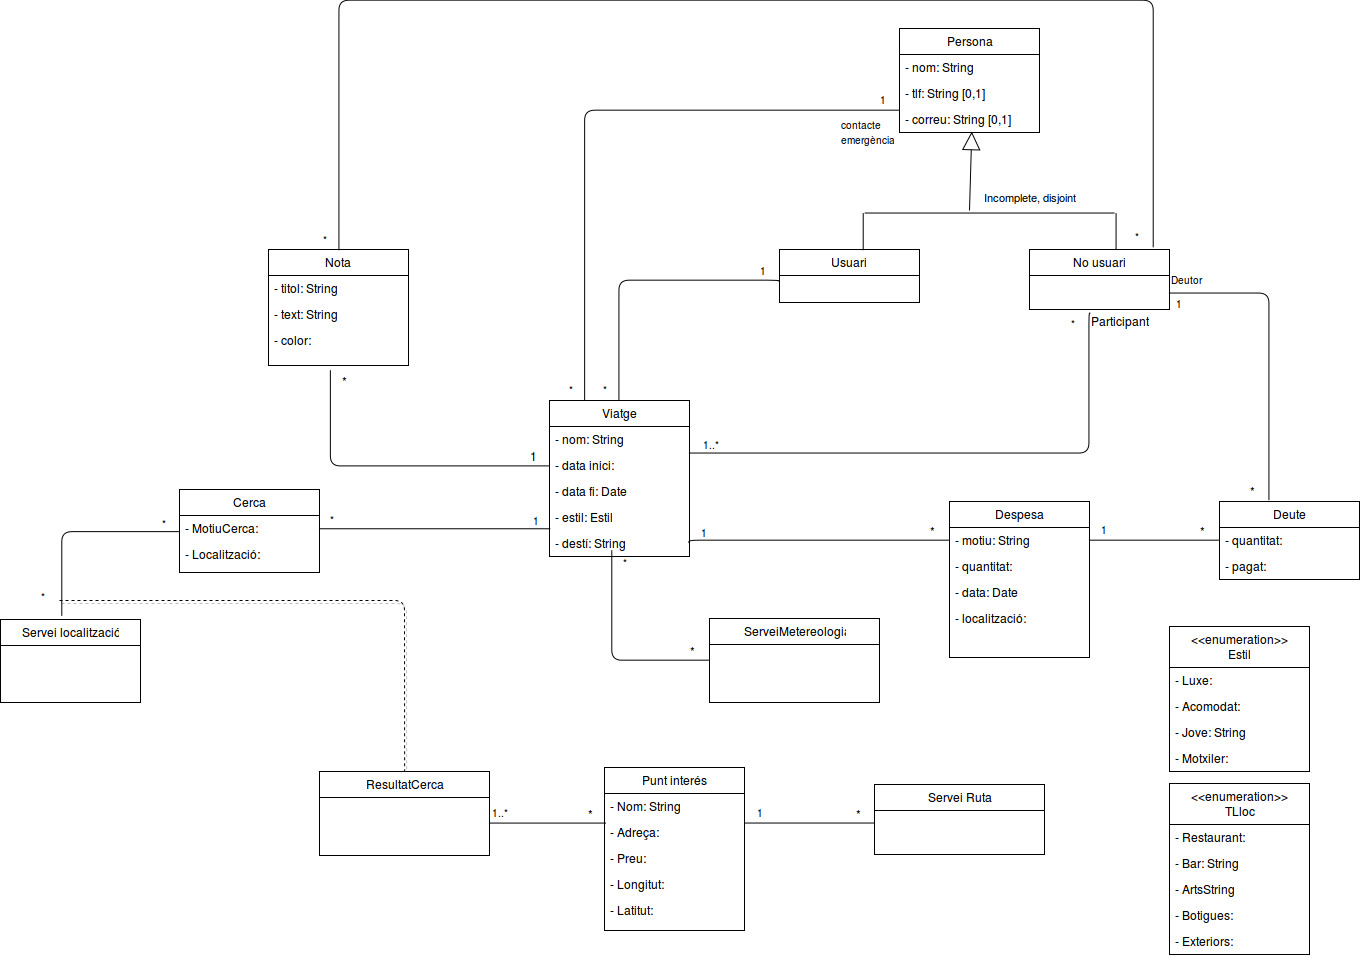
\includegraphics[scale=0.3]{Figures/UML.jpg}
\caption{Esquema conceptual.}
\end{figure}


\subsection{Restricions textuals}
\begin{itemize}
\item{}El deutor ha de ser participant del viatge al qual pertany el deute.
\item{}El viatger a qui se li comparteix una nota ha de ser participant del viatge al qual pertany la nota.
\end{itemize}

\clearpage

\subsection{Descripció de les entitats}

\newcolumntype{L}{>{\centering}m{4cm}}
\newcolumntype{M}{m{4cm}}
\newcolumntype{T}{m{7cm}}

\begin{itemize}

\item[]\textbf{Persona}\\
Super classe que s'instància per obtenir una persona de contacte.
\begin{table}[!h]
\begin{tabular}{|M|T|}
\hline
\textbf{Atribut}  & \textbf{Descripció} \\\hline
Nom &  Nom de la persona\\\hline
Tlf &  Telèfon de la persona\\\hline
Correu &  Correu electrònic de la persona\\\hline
\end{tabular}
\label{}
\caption{Atributs de la classe Persona}
\end{table}

\item[]\textbf{Usuari}\\
Té el rol d'usuari del sistema i és subclasse de Persona.
\begin{table}[!h]
\begin{tabular}{|M|T|}
\hline
\textbf{Atribut}  & \textbf{Descripció} \\\hline
Nom &  Nom de l'usuari\\\hline
Tlf &  Telèfon de l'usuari\\\hline
Correu &  Correu electrònic de l'usuari\\\hline
\end{tabular}
\label{}
\caption{Atributs de la classe Usuari}
\end{table}

\item[]\textbf{NoUsuari}\\
Té el rol de participant del viatge però sense ser usuari, no interacciona directament amb l'aplicació.

\begin{table}[!h]
\begin{tabular}{|M|T|}
\hline
\textbf{Atribut}  & \textbf{Descripció} \\\hline
Nom &  Nom del participant\\\hline
Tlf &  Telèfon del participant\\\hline
Correu &  Correu electrònic del participant\\\hline
\end{tabular}
\label{}
\caption{Atributs de la classe NoUsuari}
\end{table}

\item[]\textbf{Viatge}\\
Representa un viatge en concret, és el concepte base de l'aplicació.
\begin{table}[!h]
\begin{tabular}{|M|T|}
\hline
\textbf{Atribut}  & \textbf{Descripció} \\\hline
Nom &  Nom del viatge\\\hline
Destí &  Destí del viatge\\\hline
Data inici &  Data d'inici del viatge\\\hline
Data fi &  Data final del viatge\\\hline
Estil &  Estil de viatjar seleccionat per l'usuari\\\hline
\end{tabular}
\label{}
\caption{Atributs de la classe Viatge}
\end{table}

\clearpage

\item[]\textbf{Despesa}\\
Representa una despesa de l'usuari durant un viatge.

\begin{table}[!h]
\begin{tabular}{|M|T|}
\hline
\textbf{Atribut}  & \textbf{Descripció} \\\hline
Motiu &  Motiu de la despesa\\\hline
Quantitat &  Quantiat en euros de la despesa\\\hline
Localització &  Lloc on s'ha generat la despesa\\\hline
Data &  Data de creació de la despesa\\\hline
\end{tabular}
\label{}
\caption{Atributs de la classe Despesa}
\end{table}


\item[]\textbf{Deute}\\
Representa un deute d'un participant del viatge amb l'usuari.

\begin{table}[!h]
\begin{tabular}{|M|T|}
\hline
\textbf{Atribut}  & \textbf{Descripció} \\\hline
Quantitat & Quantitat del deute en euros.\\\hline
Pagat &  Indica si el deute ja ha estat pagat o no.\\\hline
\end{tabular}
\label{}
\caption{Atributs de la classe Deute}
\end{table}


\item[]\textbf{Nota}\\
Representa una nota escrita per l'usuari.

\begin{table}[!h]
\begin{tabular}{|M|T|}
\hline
\textbf{Atribut}  & \textbf{Descripció} \\\hline
Títol & Títol de la nota\\\hline
Text &  Text de la nota\\\hline
Color & Color que ha seleccionat l'usuari pel fons de la nota.\\\hline
\end{tabular}
\label{}
\caption{Atributs de la classe Nota}
\end{table}

\item[]\textbf{Cerca}\\
Representa una cerca llençada per l'usuari al sistema.

\begin{table}[!h]
\begin{tabular}{|M|T|}
\hline
\textbf{Atribut}  & \textbf{Descripció} \\\hline
Motiu & Tipus de cerca, aquest valor pot ser: menjar, begudes, arts, botigues o espais oberts\\\hline
Localització &  Localització des d'on es vol realitzar la cerca\\\hline
\end{tabular}
\label{}
\caption{Atributs de la classe Cerca}
\end{table}


\item[]\textbf{Servei Localització}\\
Representa el servei extern amb qui es comunica el sistema per obtenir resultats en la cerca.


\item[]\textbf{Resultat Cerca}\\
Representa els resultats d'una cerca en concret.

\item[]\textbf{Punt d'interés}\\
Representa un item concret del resultat de la cerca.

\begin{table}[!h]
\begin{tabular}{|M|T|}
\hline
\textbf{Atribut}  & \textbf{Descripció} \\\hline
Nom & Nom del punt d'interés\\\hline
Adreça &  Adreça del punt d'interés\\\hline
Preu & Nivell de preus del punt d'interés\\\hline
Latitut & Valor de latitut en la localització del punt d'interés\\\hline
Longitut & Valor de longitut en la localització del punt d'interés\\\hline
\end{tabular}
\label{}
\caption{Atributs de la classe Punt d'interés}
\end{table}


\item[]\textbf{Servei Ruta}\\
Representa el servei extern amb qui es comunica el sistema per tal d'obtenir una ruta entre dos punts.

\item[]\textbf{Servei Meteorologia}\\
Representa el servei extern amb qui es comunica el sistema per tal d'obtenir la previsió metereològica.



\end{itemize}

\section{Esquema del comportament}

